\newpage
\subsection{Electrical parameters}
\label{sec:doseditor}
The electrical parameter editor enables you to change the electrical parameters associated with the active layers. Here you can change mobilities, trap constants etc. If you set a layer to active wihtin the layer editor it will apear within the electrical paramter editor. The toolbar at the top of the window allows you to turn off and on various electrical mechanisms including:

\begin{itemize}
  \item Drift diffusion: This enabled drift diffusion within the layer. In most circumstances if a layer is set to be active there is no reason why you would want to turn this option off. The one example is in the insulating layer of an OFET.
  \item Auger recombination: This switches on and off Auger recombination. See \ref{sec:auger} for more information.
  \item Dynamic SRH traps: This is used to turn on and off dynamic SRH traps.  See section \ref{sec:SRHintro} for more information. This option should be turned on when modeling disordered semiconductors such as organic materials.
  \item Equilibrium SRH traps: This can be used to introduce a single equilibrium trap level.  See section \ref{sec:SRHintro} for more information.
  \item Excitons: This enables the exciton diffusion equation to be solved along with the electrical equations. See section \ref{sec:excitions} for more information.
  \item Excitons: This enables singlet and triplet states to be modelled.
\end{itemize}

\begin{figure}[H]
\centering
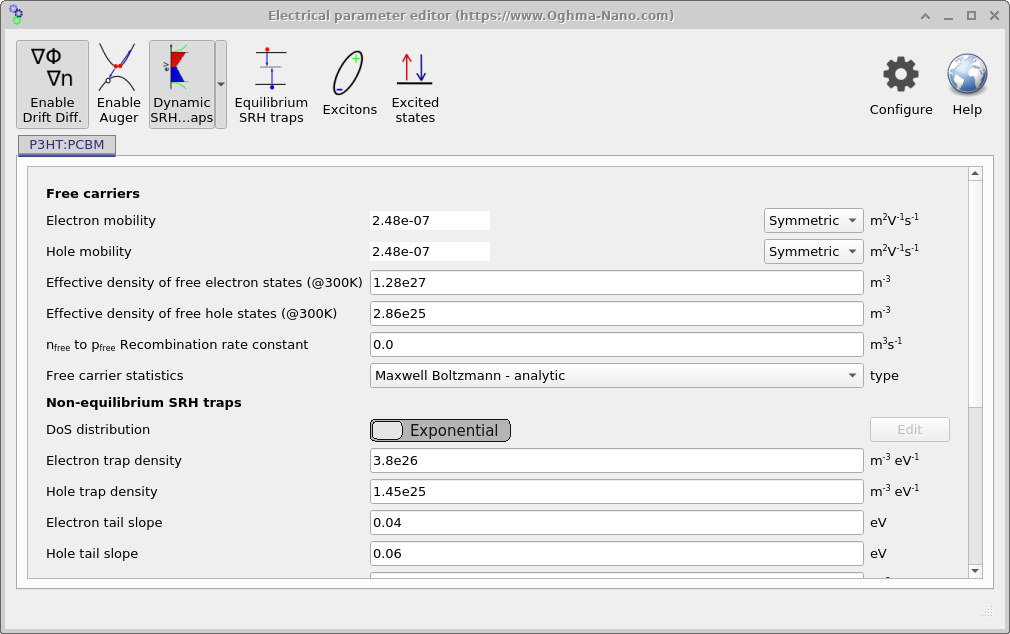
\includegraphics[width=100mm,height=70mm]{./images/running/dos_editor.png}
\caption{Electrical parameter window}
\label{fig:electricalparamwindow}
\end{figure}

\vspace*{\fill}
\fbox{
\parbox{0.9\textwidth}{
\color{blue} Task \addtocounter{question}{1}\thequestion : The values of electron mobility dictate how easily charge can move in the device.  You can think of this value as akin to resistance or a sort of microscopic resistance. Try try increasing the mobilities by two orders of magnitude and look what happens to the light JV curve of the device and the efficiency, FF, $V_{oc}$ and $J_{sc}$  Do you think it is good to have a low or high value of mobility?
}\par
}


\newpage
\fbox{
\parbox{0.9\textwidth}{
\color{blue} Task \addtocounter{question}{1}\thequestion : Recombination is described later in detail but for now we can simply think of it as how many electrons and holes meet each other in a given time. As stated above there are various types of recombination which can happen in organic semiconductors, but for now we will \emph{just consider}  the case when a free electron meets a free hole.  This is sometimes called bi-molecular recombination, the equation for this is given by:
\begin{equation}
R(x)=kn(x)p(x)
\end{equation}
Where $n(x)$ is the density of electrons and $p(x)$ is the density of holes, and k is a rate constant.  Before trying to understand this rate, firstly turn off the more complex SRH recombination by clicking on the \emph{Dynamic SRH traps} in figure \ref{fig:electricalparamwindow}.  You will notice lots of text boxes disappear. Then try changing the value of $k$ which is set in the text box called $n_{free}$ to $p_{free}$ Recombination rate constant, from 1e-15 to 1e-20 in five steps.  Run a simulation each time you change the value and make a graph of the efficiency of the cell as you change the value. 
}\par
}

\subsubsection{How do I know what electrical parameters to use?}
For traditional semiconductors that have been studied for years such as AlGaAs or InP the values of charge carrier mobility, band gap, electron  affinity (etc..) are well known and can simply be looked up on sites such as \href{https://www.ioffe.ru/SVA/NSM/Semicond/AlGaAs/index.html}{this} or in books such in Piprek's \cite{piprek2013semiconductor} excellent book. These materials are highly pure (99.999999999\%) (the so-called "eleven nines" purity). This means that when one has a sample of such a semiconductor one knows exactly what one has in the hand and what its physical properties will be. Organic semiconductors (also other novel materials such as perovskites etc..) on the are typically only 99.9\% on a good day, that is a whole eight orders of magnitude less pure than their traditional counterparts. This means that when one has a sample of such a material one is not exactly sure what material one has hold of so it's harder to know what the values of mobility etc will be.

Furthermore, traditional semiconductors are very ordered, this means that the atoms within them pack in a regular lattice (think marbles packing in a biscuit tin) this again helps make their electronic properties predictable. Novel semiconductors on the other hand are typically much more disordered than their traditional counterparts and consist of a higgldy piggidly collection of polymers/molecules (or perovskite domains etc..), and the exact structure of these materials depends very much on how they were deposited. This means that due to fabrication techniques/conditions varying between different labs, nominally the same material produced by the same suppler but can behave very differently depending on when/who/where it was deposited by.

So this brings us back to the question that started this section, what parameters should I use for my novel device? Here are some tips:

\begin{itemize}
  \item Use the base simulations provided in OghmaNano, these simulations have either been calibrated against real experimental devices or use very reasonable electrical parameters.
  \item Look in the literature and try to get an idea of what values are sensible ranges for the material systems you are looking at.
  \item Find some experimental data and make sure the current voltage curves produced by the model are within the same ball park as what you would expect experimentally, if they are totally out then you might need to tweak your electrical paramters.
  \item Fit the model to an experimental data set as was done in \cite{mackenzie2012extracting} and described in section \ref{sec:fitting} (This is however quite a hard thing to do though and not really recommended).
\end{itemize}

